\section{Experiments}
% \vspace{-1mm}
\paragraph{Dataset} Most NeRF benchmarks~\cite{guo2023streetsurf,yang2023emernerf,yan2024street} for driving focus on a single-traversal video of the Waymo~\cite{sun2020scalability} or nuScenes~\cite{caesar2020nuscenes}. To address the gap, we introduce the first \textit{unsupervised \textbf{Map}ping and segmentation via multitra\textbf{verse}} (\textbf{Mapverse}) benchmark, which comprises \textbf{Mapverse-Ithaca365} (see Appendix~\ref{subsec:ithaca-appendix}) and \textbf{Mapverse-nuPlan} (see Appendix~\ref{subsec:nuplan-appendix}) derived from the Ithaca365~\cite{diaz2022ithaca365} and nuPlan~\cite{karnchanachari2024towards} datasets, respectively. \textbf{Mapverse} features 40 locations, each with 10$\sim$16 traversals, yielding a total of 467 videos and 35,304 images. Due to space constraints, we present results for \textbf{Mapverse-Ithaca365} (20 locations, 
 200 videos, 20,000 images) in the main text, with additional results in \textbf{Mapverse-nuPlan} provided in Appendix~\ref{sec:seg-nuplan-app}\textasciitilde\ref{sec:rendering-nuplan-app}. Sample data are visualized in Figs.~\ref{fig:ithaca-1}\textasciitilde\ref{fig:nuplan-2}.

% \vspace{-2mm}
\paragraph{Task and implementation} We benchmark three tasks: \emph{(1)} \textit{{unsupervised 2D ephemerality segmentation}}, \emph{(2)} \textit{{3D reconstruction}}, and \emph{(3)} \textit{{neural rendering}} in multitraversal driving. Our benchmark can inspire wide applications in unsupervised perception, autolabeling, camera-only 3D reconstruction and neural simulation in self-driving and robotics. For efficiency, we compress feature dimensions from 768 to 64 using PCA. Our model uses KL divergence for feature alignment and L1 loss for RGB reconstruction. All experiments are conducted on a single NVIDIA RTX 3090 GPU.

% \vspace{-2mm}
\subsection{Unsupervised 2D Ephemeral Object Segmentation}
% \vspace{-1mm}
\paragraph{Task setup} Our \texttt{EmerSeg} can segment ephemeral traffic participants in a multitraverse image collection, \textit{without any supervision}. This will help identify moving objects like vehicles and pedestrians, as well as static objects with the potential for movement, such as parked cars or traffic cones. We use a \textit{training-as-optimization} pipeline and adopt the \textit{Intersection over Union (IoU) metric} for evaluation. Regarding comparison methods, we employ several state-of-the-art \textit{semantic segmentation} models trained with human annotations to create pseudo ground-truth masks for transient objects  (pedestrians, vehicles, bicyclists, and motorcyclists). We also compare \texttt{EmerSeg} with \textit{unsupervised segmentation} methods. We report the main comparison results in Sec.~\ref{subsubsec:main-seg} and ablation studies in Sec.~\ref{subsubsec:ablation-seg}.
% \vspace{-2mm}
\subsubsection{Quantitative and Qualitative Evaluations}
\label{subsubsec:main-seg}
% \vspace{-1mm}
\paragraph{Comparison against supervised methods} We compare our method with state-of-the-art (SOTA) semantic segmentation methods: PSPNet~\cite{zhao2017pyramid}, SegViT~\cite{zhang2022segvit}, 
Mask2Former~\cite{cheng2022masked}, SegFormer~\cite{xie2021segformer}, and InternImage~\cite{wang2023internimage}. \textit{Note that these methods require dense pixel-level annotations to learn semantics.} We directly use these models trained on either ADE20K~\cite{zhou2017scene} or Cityscapes~\cite{cordts2016cityscapes} to produce masks on \textbf{Mapverse-Ithaca365}. The overall IoU scores of \texttt{EmerSeg} average around 0.45 compared to the five supervised models; see Tab.~\ref{tab:main-seg}. IoU scores across 20 locations are detailed in Fig.~\ref{fig:iouvsloc}, with seven locations surpassing 50\% IoU, and the highest score reaching 56\% compared to SegFormer. These results highlight the promising potential of our unsupervised segmentation paradigm.
% \vspace{-2mm}
\paragraph{Comparison against unsupervised methods} We compare \texttt{EmerSeg} with two SOTA unsupervised segmentation methods, \textit{i.e.}, STEGO~\cite{hamilton2022unsupervised} and CAUSE~\cite{kim2023causal}. We train both methods on our dataset using their unsupervised objectives. \textit{Note that these unsupervised baseline methods cannot grasp the semantics or the concept of ephemerality and can only perform clustering within a single image.} Following prior work, we use a Hungarian matching algorithm to align the unlabeled clusters with pseudo ground-truth masks for evaluation. As shown in Tab.~\ref{tab:main-seg}, \texttt{EmerSeg} significantly outperforms STEGO and CAUSE, with a 21.36-point (89.8\%) IoU improvement over STEGO using SegFormer masks. More importantly, \texttt{EmerSeg} can understand ephemerality, a capability lacking in prior works.


\begin{figure}[tb]
  \centering
  \begin{minipage}[t]{0.525\textwidth}
\scriptsize
\centering
\captionof{table}{\textbf{Mean IoU of unsupervised vs. five supervised methods in Mapverse-Ithaca365.} $^*$~indicates the model without training on our dataset.}
% \vspace{3mm}Cityscapes
\label{tab:main-seg}
\renewcommand{\arraystretch}{1.1}
% \resizebox{0.99\textwidth}{!}{
\setlength{\tabcolsep}{1.6mm}{
\begin{tabular}{ccccc}
\toprule
\multirow{2}{*}{\diagbox{\textbf{Sup.}}{\textbf{Unsup.}}} & \textbf{EmerSeg} & \textbf{STEGO$^*$} & \textbf{STEGO} & \textbf{CAUSE} \\
& \textbf{(Ours)} & \cite{hamilton2022unsupervised} & \cite{hamilton2022unsupervised} & \cite{kim2023causal}\\
\midrule
\textbf{PSPNet}~\cite{zhao2017pyramid} & \textbf{42.22} &20.55 & 22.22& 19.12 \\
\textbf{SegViT}~\cite{zhang2022segvit} & \textbf{46.16} & 21.18 & 23.57& 19.64 \\
\textbf{InternImage}~\cite{wang2023internimage} & \textbf{46.34} & 21.29&23.68 & 19.93 \\
\textbf{Mask2Former}~\cite{cheng2022masked} & \textbf{42.28} & 20.83 &23.03& 20.88 \\
\textbf{SegFormer}~\cite{xie2021segformer} & \textbf{45.14} & 21.31 &23.78& 20.63 \\
\bottomrule
\end{tabular}
}
  \end{minipage}%
  \hfill
  \begin{minipage}[t]{0.475\textwidth}
    \vspace{0pt} % Ensure alignment at the top
    \centering
    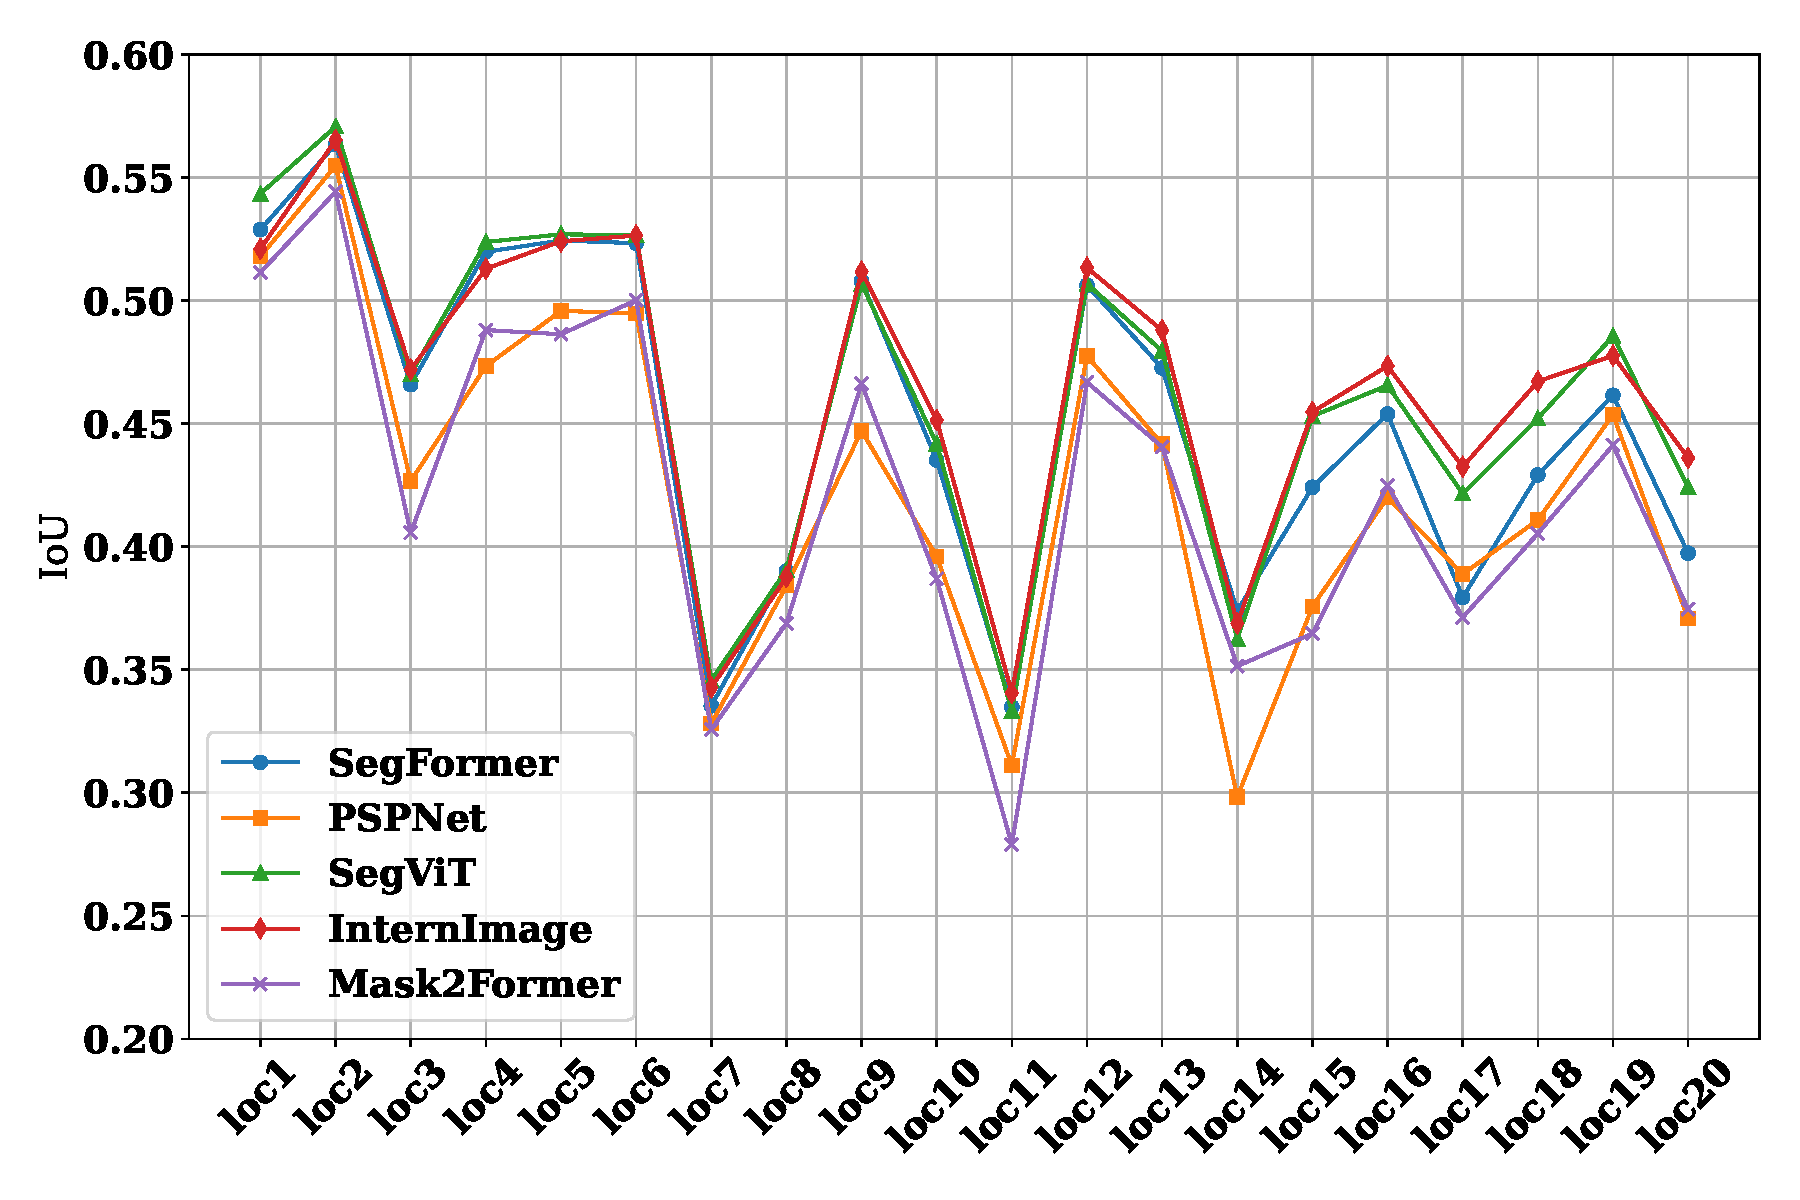
\includegraphics[width=0.88\textwidth]{figs_compressed/seg-loc.pdf}
     \vspace{-3mm}
    \caption{\small{\textbf{IoU at 20 locations in Ithaca, NY.}}}
    \label{fig:iouvsloc}
  \end{minipage}
  % \vspace{3mm}
\end{figure}



\paragraph{Qualitative comparison} \texttt{EmerSeg} performs well in various lighting and weather conditions, effectively segmenting cars, buses, and pedestrians; see Fig.~\ref{fig:vis-seg}. However, it struggles with small or distant objects due to low feature map resolution. \textit{We empirically find that small objects have minimal impact on neural rendering as they occupy few pixels.} Additional qualitative results are in Fig.~\ref{fig:visseg-appendix}, with visualizations of baseline methods in Fig.~\ref{fig:comparison-seg-appendix}. Detailed limitations are discussed in Appendix~\ref{sec:limitation-appendix}.

% \vspace{-2mm}

\paragraph{Computation time} Figure~\ref{fig:ablation-iteration-appendix} illustrates the convergence of our segmentation method, showing a rapid increase in IoU during the initial iterations, which stabilizes around iteration 4,000. Notably, a resolution of 110×180 requires only 2,000 iterations to achieve an IoU score exceeding 40\%, taking  $\sim$8 minutes on a single NVIDIA RTX 3090 GPU for 1,000 images from 10 traversals of a location.
% \vspace{-1mm}

\subsubsection{Ablation Studies}
% \vspace{-1mm}
\label{subsubsec:ablation-seg}
\paragraph{Segmentation performance benefits from more traversals} We evaluate 2D segmentation on 100 images from a single traversal, using inputs from varying numbers of traversals; see Tab.\ref{tab:seg-ablation}. Starting at 15.15\% with one traversal, the IoU jumps to 42.31\% with two, and continues to rise: 53.16\% at 8 and 56.01\% at 10 traversals. This shows a clear trend of improving IoU with more traversals, with significant gains between 1 and 2. Detailed visualizations are in Fig.~\ref{fig:ablation-traversal-appendix}.

% \vspace{-2mm}
\paragraph{Effective segmentation requires 32 feature dimensions} We use PCA to compress the dimensions of DINOv2 features to save computation and storage. Our tests on segmentation performance at various dimensions revealed that 32 is an approximate threshold; IoU scores decrease significantly to around 10\%-25\% when the number of dimensions falls below 32, as shown in Tab.~\ref{tab:seg-ablation}. Qualitative comparisons of different feature dimensions are demonstrated in Fig.~\ref{fig:ablation-dimension-appendix}.

% \vspace{-2mm}
\paragraph{A resolution of 70×110 can achieve an IoU $>$40\%} Table~\ref{tab:seg-ablation} shows IoU at various feature resolutions and sizes. IoU improves significantly as resolution increases from 25×40 (28.61\%, 0.3 MB) to 110×180 (44.13\%, 5.0 MB). However, higher resolutions like 140×210 and 160×260 result in slightly lower IoU scores of 42.48\% and 41.19\%, despite larger sizes. This indicates an optimal resolution at 110×180, balancing accuracy and efficiency. Visualizations at different resolutions are in Fig.~\ref{fig:ablation-resolution-appendix}.

% \vspace{-2mm}
\paragraph{Vision foundation model matters in unsupervised segmentation} We use robust features from self-supervised vision foundation models like DINO~\cite{caron2021emerging}, DINOv2~\cite{oquab2023dinov2}, and DINOv2 with registers~\cite{darcet2023vision}. Additionally, we employ DVT~\cite{yang2024denoising} to reduce grid-like artifacts in ViT feature maps. As shown in Tab.~\ref{tab:seg-ablation}, Denoised DINOv2 outperforms other models, highlighting the importance of robust, discriminative features for identifying transient clusters. Detailed visualizations are in Fig.~\ref{fig:ablation-backbone-appendix}.



\begin{figure}[t]
\begin{center}
\centerline{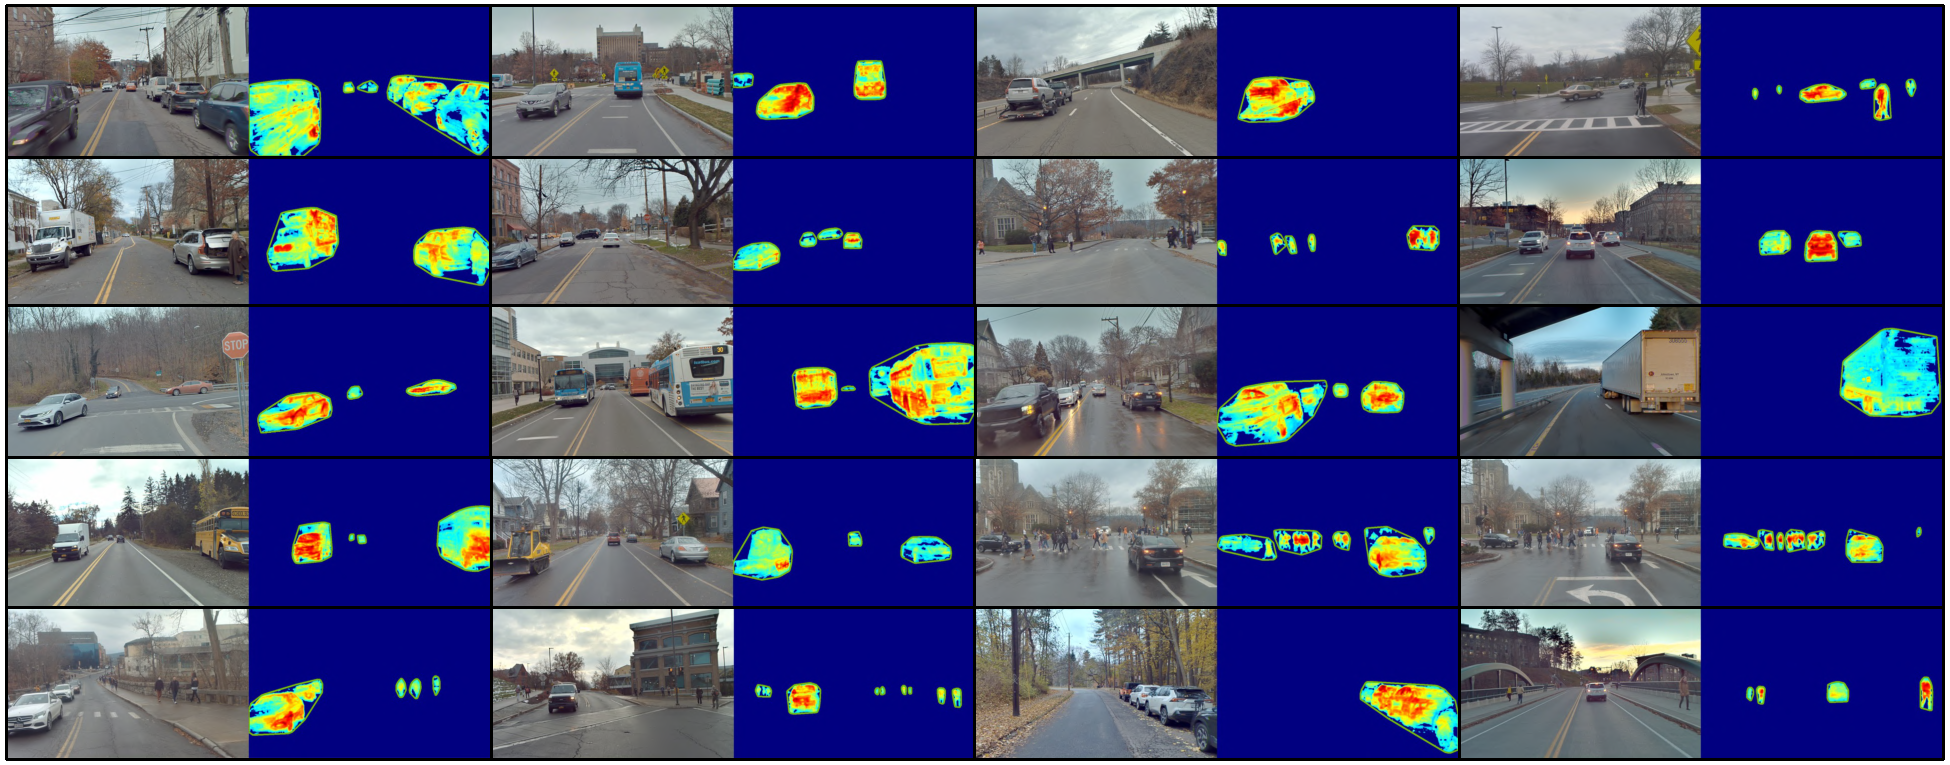
\includegraphics[width=0.99\columnwidth]{figs_compressed/featmask_compressed.pdf}}
% \vspace{-1mm}
\caption{\textbf{Qualitative evaluations of \texttt{EmerSeg} in Mapverse-Ithaca365.}}
\label{fig:vis-seg}
\end{center}
\vspace{-5mm}
\end{figure}


\begin{table}[t]
\scriptsize
\centering
\caption{\textbf{Ablation Study Results of \texttt{EmerSeg} in Mapverse-Ithaca365.}}
\label{tab:seg-ablation}
% \resizebox{\textwidth}{!}{ 
\setlength{\tabcolsep}{1.2mm}{
\begin{tabular}{cc|ccc|ccc|cc}
\toprule
\multicolumn{2}{c|}{\textbf{Number of Traversals}} & \multicolumn{3}{c|}{\textbf{Feature Dimension}} & \multicolumn{3}{c|}{\textbf{Feature Resolution}} & \multicolumn{2}{c}{\textbf{Feature Backbone}} \\
\midrule
\textbf{\#} & \textbf{IoU (\%)} & \textbf{Dim.} & \textbf{Runtime} & \textbf{IoU (\%)} & \textbf{Res.} & \textbf{Size (MB)}& \textbf{IoU (\%)} & \textbf{Backbone} & \textbf{IoU (\%)} \\
\midrule
1 & 15.15  & 4 & 00:13:50 & 9.45& 25$\times$40 & 0.3 & 28.61 & DINO~\cite{caron2021emerging} & 16.51 \\
2 & 42.31 & 8 & 00:16:50 & 10.91 & 50$\times$80 & 1.0 & 35.91 &Denoised DINO~\cite{yang2024denoising} & 14.95  \\
3 & 46.62 & 16 & 00:18:37 & 26.32 & 70$\times$110 & 1.9 & 40.09 & DINOv2~\cite{oquab2023dinov2} & 35.14  \\
5 & 53.68 & 32 & 00:24:48 & 37.51 & 110$\times$180& 5.0 & \textbf{44.13} & Denoised DINOv2~\cite{yang2024denoising} & \textbf{44.13}  \\

9 & 54.50 & 64 & 00:40:25 & \textbf{44.13} & 140$\times$210& 7.4 & 42.48 & DINOv2-reg~\cite{darcet2023vision} & 23.51  \\

10 & \textbf{56.01} & 128 & 01:13:53 & 42.55 & 160$\times$260& 10.5 & 41.19 & Denoised DINOv2-reg~\cite{yang2024denoising} & 36.30  \\
\bottomrule
\end{tabular}
}
% \vspace{-3mm}
\end{table}


\subsection{3D Environment Reconstruction}
\label{subsec:reconstruction}
\paragraph{Task setup} Our \texttt{EnvGS} can extract 3D points from Gaussian Splatting, enabling the reconstruction of 3D environments from camera-only input while effectively ignoring transient objects across repeated traversals. We utilize a \textit{training-as-optimization} pipeline and employ the \textit{Chamfer Distance (CD) metric} for quantitative evaluation. For our comparison baseline, we use the state-of-the-art DepthAnything~\cite{depthanything} model, which is trained with a combination of LiDAR ground truth (GT) depth data and unlabeled image data. This approach ensures that DepthAnything leverages diverse data sources to achieve satisfactory performance in zero-shot depth estimation.

% \vspace{-2mm}

\paragraph{Quantitative results} Figure~\ref{fig:depth} demonstrates the large reduction in Chamfer Distance (CD) achieved by \texttt{EnvGS} across nearly all locations. Our method achieves an average CD of approximately 0.9 meters, showcasing its precision in 3D reconstruction. Notably, there are five locations where the CD is even lower than 0.5 meters, highlighting the good accuracy of our approach in these areas. In contrast, DepthAnything has an average CD of around 1.9 meters, indicating a notable performance gap between the two methods. More importantly, our method avoids the need for costly LiDAR sensors during training, making it a cost-effective autonomous mapping solution for self-driving and robotics. Leveraging techniques such as mesh reconstruction~\cite{guedon2023sugar} and 2D Gaussian Splatting~\cite{Huang2DGS2024} could further enhance the geometric reconstruction capabilities of our method.

% \vspace{-2mm}

\begin{figure}[t]
    \centering
    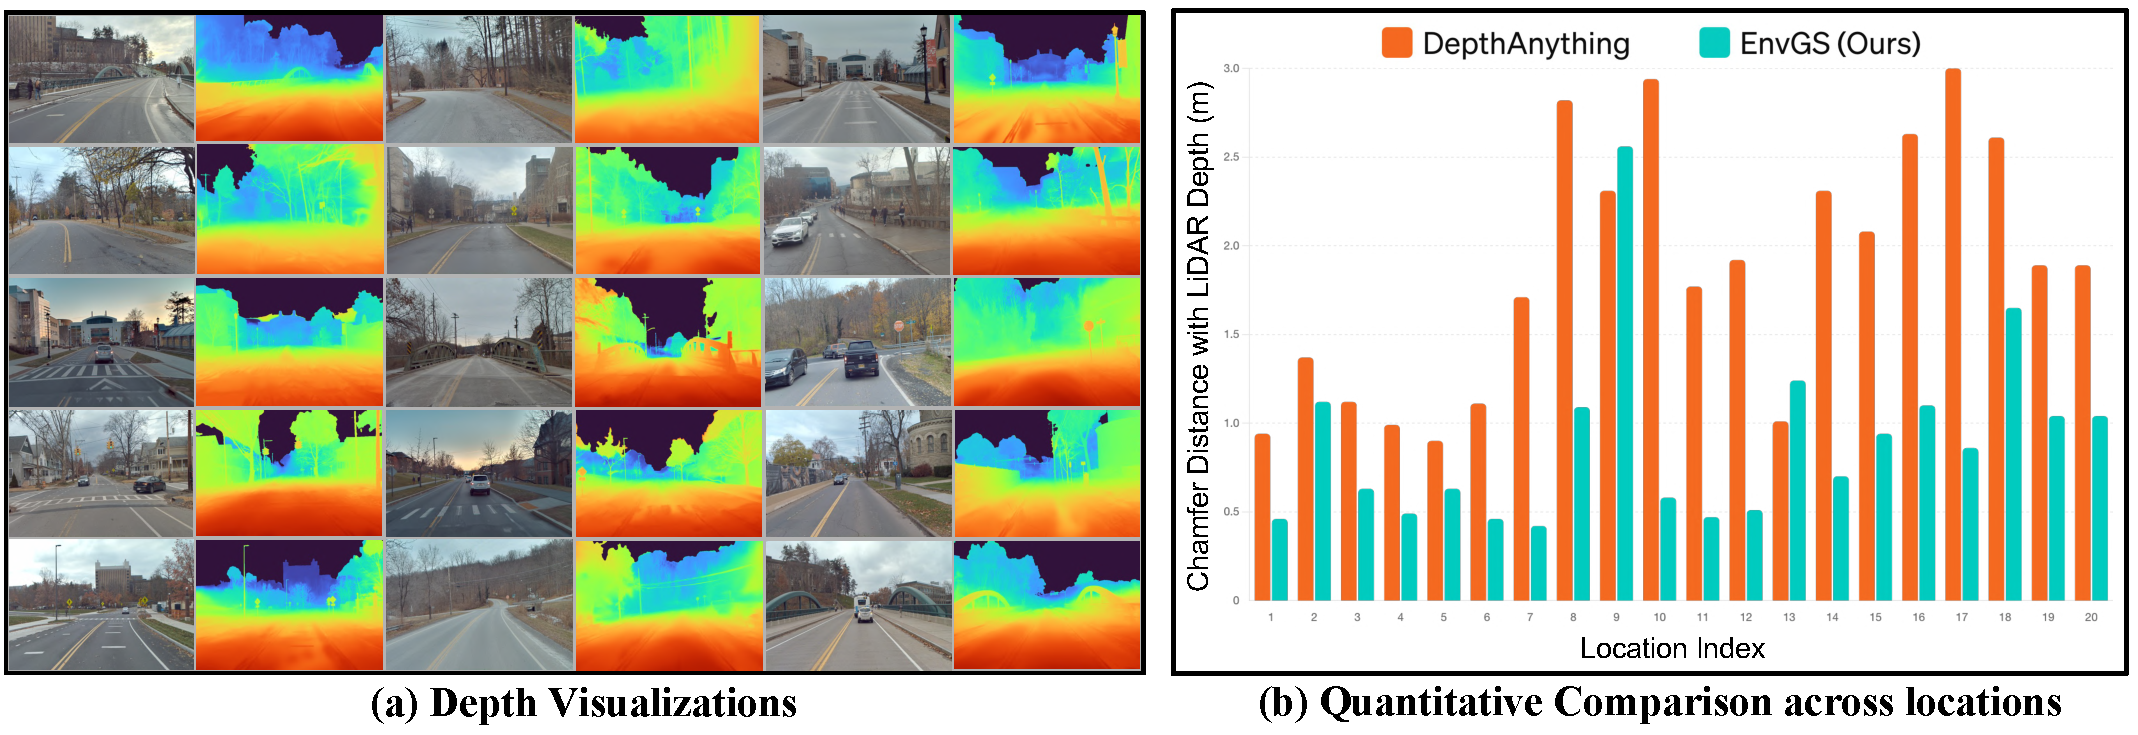
\includegraphics[width=\linewidth]{figs_compressed/depth_comb_compressed.pdf}
    \caption{\textbf{Qualitative and quantitative evaluation of 3D geometry in Mapverse-Ithaca365.}}
    \label{fig:depth}
    % \vspace{-3mm}
\end{figure}

\paragraph{Qualitative results} Figure~\ref{fig:depth} showcases depth visualizations of \texttt{EnvGS} across various driving scenarios. The depth maps generated by \texttt{EnvGS} exhibit superior accuracy, with smooth transitions from near to far objects and well-defined edges of scene structures. Additionally, \texttt{EnvGS} effectively removes transient objects without human supervision. Visualizations in 3D are shown in Fig.~\ref{fig:reconstruction-appendix}. 




% \vspace{-2mm}
\subsection{Neural Environment Rendering}
% \vspace{-1mm}

\paragraph{Task setup}
Our \texttt{EnvGS} can also achieve novel view synthesis through splatting-based rasterization. The challenge lies in ensuring the environment rendering automatically bypasses the non-environment pixels, \textit{i.e.}, transient objects.
We evaluate the quality of rendered images using three metrics: Learned Perceptual Image Patch Similarity (LPIPS), Structural Similarity Index (SSIM), and Peak Signal-to-Noise Ratio (PSNR). Given the absence of ground truth RGB images for clean backgrounds, we utilize the pretrained SegFormer~\cite{xie2021segformer} model to isolate foreground regions, allowing us to focus our evaluation exclusively on the quality of the background rendering.

% \vspace{-2mm}

\paragraph{Baseline methods} Our baseline methods include two NeRF-based methods, leveraging the implementation framework of iNGP~\cite{muller2022instant}. The first, VanillaNeRF, constructs the scene within a single, static hash table and directly learns grid features from multitraverse images. In contrast, RobustNeRF~\cite{sabour2023robustnerf} introduces an adaptive weighting mechanism to filter out outliers. In addition to the original 3DGS framework, we introduce two 3DGS-based baseline methods. 3DGS+RobustNeRF integrates the loss function from RobustNeRF, and 3DGS+SegFormer utilizes masks generated by a supervised segmentation model. For a fair comparison, all methods exclusively rely on camera images as input.

% \vspace{-2mm}
% Furthermore, consistent with the original EmerNeRF implementation, NeRF-based methods employ a sky mask.

\paragraph{Results and discussions} Table~\ref{tab:rendering} presents a quantitative comparison of various methods, showing that 3DGS-based approaches outperform NeRF-based methods. Adding the RobustNeRF loss function does not improve rendering quality in driving scenes. However, incorporating SegFormer or EmerSeg masks achieves the best LPIPS and SSIM. This is notable within a purely self-supervised framework, showcasing the potential of our self-supervised paradigm in pushing the boundaries of neural mapping. We present qualitative examples in Fig.~\ref{fig:visenv}, where it is evident that the original 3DGS model struggles with accurately reconstructing background regions affected by transient objects. More interestingly, our method can identify and mask out not only the objects themselves but also their associated non-environmental elements, such as shadows, as shown in the third and sixth columns of Fig.~\ref{fig:visenv}. More qualitative examples can be found in Fig.~\ref{fig:rendering-appendix}.



% \vspace{-2mm}
\section{Conclusion}
\label{sec:conclusion}
% \vspace{-1mm}
\paragraph{Broader impacts}
The concept of vision-only neural representation learning through repeated traversals extends beyond object segmentation and environment mapping, benefiting the vision and robotics communities. With a neural map prior, our approach becomes a powerful self-supervised framework for change detection and object discovery. This capability to render and analyze multitraverse environments over time is crucial for identifying environmental changes, aiding in early intervention for deforestation, urban expansion, or post-disaster assessments. Additionally, our method can serve as a baseline for autolabeling 2D masks and has potential for 3D autolabeling with LiDAR integration.

\paragraph{Limitations}
Our method faces limitations in modeling large environmental variations, including nighttime conditions, major seasonal shifts, and adversarial weathers. We also note the presence of noise in the segmentation outputs caused by motion blur or appearance shifts. Leveraging temporal information or more powerful vision foundation models could help address this issue. More discussions can be found in Appendix~\ref{sec:limitation-appendix}.

\paragraph{Summary} We introduce \texttt{3D Gaussian Mapping (3DGM)}, a novel self-supervised, camera-only framework that utilizes repeated traversals for simultaneous 3D environment mapping (\texttt{EnvGS}) and 2D unsupervised object segmentation (\texttt{EmerSeg}). Additionally, we develop the \textbf{Mapverse} benchmark, comprising nearly 500 driving video clips from the Ithaca365 and nuPlan datasets. Our method's effectiveness in unsupervised 2D segmentation, 3D reconstruction, and neural rendering is validated through both qualitative and quantitative assessments in repeated driving scenarios. Furthermore, \texttt{3DGM} opens new research opportunities, such as online unsupervised object discovery and offline autolabeling. We believe our work will advance vision-centric and learning-based self-driving and robotics, setting new standards in multitraverse setups and self-supervised scene understanding.

\begin{figure}[t]
\begin{center}
\centerline{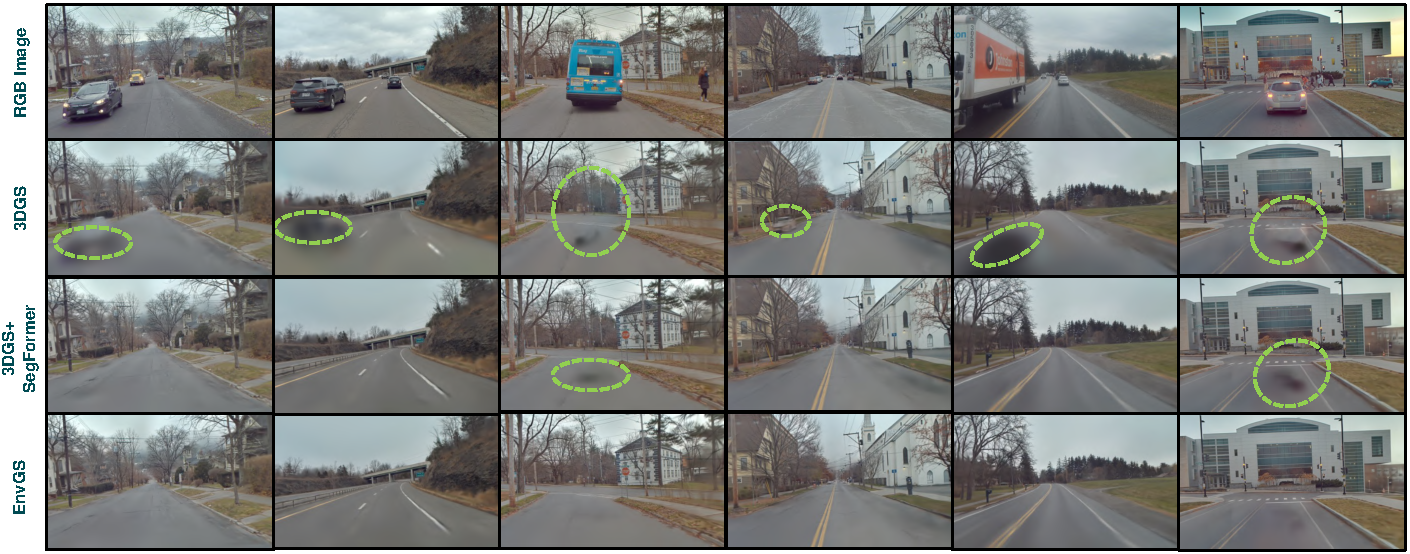
\includegraphics[width=\columnwidth]{figs_compressed/envrendering_compressed.pdf}}
\caption{\textbf{Qualitative evaluations of the environment rendering.} Our method demonstrates robust performance against transient objects, and can even outperform the method equipped with a pretrained model in some cases. Notably, this includes the effective removal of object shadows.}
\label{fig:visenv}
\end{center}
\vspace{-5mm}
\end{figure}

\begin{table}[t]
    \scriptsize
    % \small
    \centering
    \captionof{table}{\textbf{Quantitative evaluation of novel view synthesis.} We set test/training views as 1/8. Pixels corresponding to transient objects are removed in the evaluations since we do not have ground truth background pixels in these regions occluded by transient objects.}
    \label{tab:rendering}
    % \renewcommand{\arraystretch}{1.1} % Adjust the 1.5 factor as needed to increase row height
    \resizebox{\textwidth}{!}{
    \begin{tabular}{@{}ccccccc@{}}
      \toprule 
       \textbf{Metrics $\backslash$ Methods } & {\textbf{VanillaNeRF}~\cite{muller2022instant}} & {\textbf{RobustNeRF}~\cite{sabour2023robustnerf}} &  {\textbf{3DGS+RobustNeRF}} & {\textbf{3DGS}~\cite{kerbl20233d}} & {\textbf{3DGS+SegFormer}} & {\textbf{EnvGS (Ours)}} \\
      \midrule
      \textbf{LPIPS} ($\downarrow$) & 0.423 & 0.443  & 0.416 & 0.227 & {0.212} & 0.213 \\ % Example values
                                   \textbf{SSIM} ($\uparrow$) & 0.603 & 0.609  & 0.654 & 0.798	 & {0.806} & {0.806} \\ % Example values
                                   \textbf{PSNR} ($\uparrow$) & 19.18 & 19.22  & 19.97 & {22.92} & 22.81 & 22.78 \\ % Example values
      \bottomrule
    \end{tabular}
    }
    \vspace{-2mm}
\end{table}
